\documentclass{standalone}

\usepackage{tikz}

\begin{document}
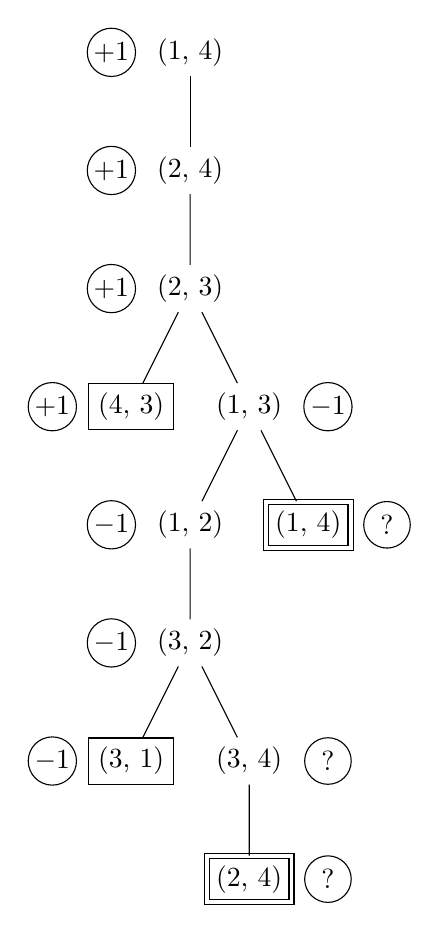
\begin{tikzpicture}[
        term/.style={rectangle, draw, text centered},
        loop/.style={rectangle, draw, double, double distance=0.5mm, text centered},
        eval/.style={circle, draw, inner sep=1pt, text centered}
    ]
    \node (init) {(1, 4)}
    child {
            node (A1) {(2, 4)}
            child {
                    node (B1) {(2, 3)}
                    child { node[term] (A21) {(4, 3)} }
                    child {
                            node (A22) {(1, 3)}
                            child {
                                    node (B21) {(1, 2)}
                                    child {
                                            node (A3) {(3, 2)}
                                            child { node[term] (B31) {(3, 1)} }
                                            child {
                                                    node (B32) {(3, 4)}
                                                    child { node[loop] (A4) {(2, 4)} }
                                                }
                                        }
                                }
                            child { node[loop] (B22) {(1, 4)}}
                        }
                }
        }
    ;
    \node[eval, left of=init] {$+1$};
    \node[eval, left of=A1]   {$+1$};
    \node[eval, left of=B1]   {$+1$};
    \node[eval, left of=A21]  {$+1$};
    \node[eval, left of=B21]  {$-1$};
    \node[eval, left of=A3]   {$-1$};
    \node[eval, left of=B31]  {$-1$};
    \node[eval, right of=A22] {$-1$};
    \node[eval, inner sep=3pt, right of=B22] {?};
    \node[eval, inner sep=3pt, right of=B32] {?};
    \node[eval, inner sep=3pt, right of=A4]  {?};
\end{tikzpicture}
\end{document}

